\chapter{CHAPTER TWO: Generalized Pochammer-Chree Equations} \label{chapter_2}

\section{Introduction}

The propagation of longitudinal deformation waves in elastic rods is governed
(\cite{LCZ}, \cite{Runz}, \cite{WM}) by 
\eqref{eq:GPC1} and \eqref{eq:GPC2},
corresponding to different constitutive relations.

References \cite{LCZ}, \cite{Runz}, \cite{WM} also discuss the primary
references, including derivations and applications of these equations in
various fields. In addition, motivated by experimental and numerical results,
there are derivations of special families of solitary wave solutions by the
extended $Tanh$ method \cite{LCZ}, and other ansatzen \cite{WM}. These extend
earlier solitary wave solutions given by Bogolubsky \cite{Bogo} and Clarkson
et. al \cite{CLVS} for special cases of \eqref{eq:GPC1} and \eqref{eq:GPC2}. In
addition, \cite{Runz} generalizes the existence results in \cite{Sax} for
solitary waves of \eqref{eq:GPC1} and \eqref{eq:GPC2}.  

\section{Solitary waves: local bifurcation}

Solitary waves of \eqref{eq:GPC1} and \eqref{eq:GPC2} of the form 
$v(x,t) = \phi\left(x - c t\right) = \phi\left(z\right)$
 satisfy the fourth-order traveling wave ODE
\begin{equation} \label{eq:ode} \phi_{zzzz} - q \phi_{zz} + p \phi = \mathcal{N}_{1,2}[\phi]
\end{equation}

where 
\begin{subequations}
\begin{eqnarray}
\mathcal{N}_1\left[\phi\right] &=& - \frac{1}{c^2}\left[  3 a_3 \left( 2 \phi \phi_z^2 + \phi^2 \phi_{zz} \right) + 2 a_2\left( \phi_{zz} \phi_z + \phi_z^2\right) \right] \\
\mathcal{N}_2\left[\phi\right] &=& - \frac{1}{c^2}\left[ 3 a_3 \left( 2 \phi \phi_z^2 + \phi^2 \phi_{zz}\right) + 5 a_5 \left( 4 \phi^3 \phi_z^2 + \phi^4 \phi_{zz} \right) \right]
\end{eqnarray}
\end{subequations}

\begin{subequations}
\begin{eqnarray}
z &\equiv& x - c t\\
p &\equiv& 0\label{eq:pdef} \\
q &\equiv & 1 - \frac{a_1}{c^2} \label{eq:qdef} 
\end{eqnarray}
\end{subequations}

Equation \eqref{eq:ode} is invariant under the transformation $ z \mapsto -z $ and is thus a reversible system. In this section we shall
use the theory of reversible systems to characterize the homoclinic orbits to the fixed point of \eqref{eq:ode}, which correspond to pulses
or solitary waves of \eqref{eq:GPC1} and \eqref{eq:GPC2} in various regions of the $(p,q)$ plane.

The linearized system corresponding to \eqref{eq:ode}
\begin{equation}
 \label{eq:linode} \phi_{zzzz} - q \phi_{zz} + p \phi = 0
\end{equation}
has a fixed point \begin{equation}\label{eq:fp} \phi = \phi_z = \phi_{zz} = \phi_{zzz} = 0 \end{equation}

Solutions $\phi = k e^{\lambda x}$ satisfy the characteristic equation
$\lambda^4 - q \lambda^2 + p = 0 $ from which one may deduce that the structure
of the eigenvalues is distinct in two regions of $\left(p,q\right)$-space.
Since $p=0$ we have only two possible regions of eigenvalues.  We denote $C_0$
as the positive $q$ axis and $C_1$ the negative $q$-axis. First we shall 
consider the bounding curves $C_0$ and $C_1$ and their neighborhoods, then we shall discuss the possible
occurrence and multiplicity of homoclinic orbits to \eqref{eq:fp}, corresponding
to pulse solitary waves of \eqref{eq:GPC1} and \eqref{eq:GPC2}, in each region:

\begin{description}
\item[Near $C_0$] 
The eigenvalues have the structure $\lambda_{1-4} = 0,0,\pm \lambda$, ($\lambda \in \mathbb{R}$) and the fixed point
\eqref{eq:fp} is a saddle-focus.
\item[Near $C_1$] 
Here the eigenvalues have the structure $\lambda_{1-4} = 0,0,\pm i \omega $, ($\omega \in \mathbb{R}$) . We will show by analysis of a
four-dimensional normal form in Section 2.4 that there exists a $\mathrm{sech}^2$ homoclinic orbit near $C_1$.
\end{description}

Having outlined the possible families of orbits homoclinic to the fixed point \eqref{eq:fp} of \eqref{eq:linode},
corresponding to pulse solitary waves of \eqref{eq:GPC1} and \eqref{eq:GPC2}, we now derive normal forms near the transition curves $C_0$ and $C_1$
to confirm the existence of regular or delocalized solitary waves in the corresponding regions of $\left(p,q\right)$ parameter space.


\section{Normal form near $C_0$: solitary wave solutions}

Using \eqref{eq:linode}, the curve $C_0$, corresponding to $\lambda = 0,0,\pm \tilde{ \lambda } $, is given by
\begin{equation}
C_0: { p=0, q > 0 }
\end{equation}

Using \eqref{eq:qdef} implies
\begin{equation}
a_1 < c^2 
\end{equation}

Denoting $\phi$ by $y_1$, \eqref{eq:ode} may be written as the two systems
\begin{subequations}\label{eq:nonbilinearsystem}
\begin{eqnarray}
\frac{d y_1 }{d z} &=& y_2 \\
\frac{d y_2 }{d z} &=& y_3 \\
\frac{d y_3 }{d z} &=& y_4 \\
\frac{d y_4 }{d z} &=& q y_3 - p y_1 - N_{1,2}(Y)
\end{eqnarray}
\end{subequations}

where
\begin{subequations}
\begin{eqnarray}
\mathcal{N}_1\left(Y\right) &=& - \frac{1}{c^2}\left[  3 a_3 \left( 2 y_1 y_2^2 + y_1^2 y_3 \right) + 2 a_2\left( y_3 y_2 + y_2^2\right) \right] \\
\mathcal{N}_2\left(Y\right) &=& - \frac{1}{c^2}\left[ 3 a_3 \left( 2 y_1 y_2^2 + y_1^2 y_3\right) + 5 a_5 \left( 4 y_1^3 y_2^2 + y_1^4 y_3 \right) \right]
\end{eqnarray}
\end{subequations}

We wish to rewrite \eqref{eq:nonbilinearsystem} as a first order reversible system in order to invoke the relevant theory \cite{IA}. 


To that end, defining  $Y=\left<y_1,y_2,y_3,y_4\right>^T$ equation 
\eqref{eq:nonbilinearsystem} can be written
\begin{equation}\label{eq:matrixeq1}
 \frac{ dY }{ dz } = A Y - G_{1,2}(Y,Y)
\end{equation}
where 
\begin{equation}\label{eq:nonlinear}
A = \left(\begin{array}{cccc}0&1&0&0\\0&0&1&0\\0&0&0&1\\-p&0&q&0\end{array}\right) 
\end{equation}
\begin{equation}\label{eq:nonlinear}
G_{1,2}(Y,Y) = \left<0,0,0,-\mathcal{N}_{1,2}\left(Y\right)\right>^T
\end{equation}

The matrix $A$ may be split into $A = L_0 + L_1 $, where 
\begin{subequations}
\begin{eqnarray}
L_0 &=& \left(\begin{array}{cccc}0&1&0&0\\0&0&1&0\\0&0&0&1\\0&0&0&0\end{array}\right) \\
L_1 &=& \left(\begin{array}{cccc}0&0&0&0\\0&0&0&0\\0&0&0&0\\-p&0&q&0\end{array}\right) 
\end{eqnarray}
\end{subequations}
We now derive a linear operator $L_{pq}$ which is equivalent to $A=L_0+L_1$ and in reversible form.

Let $L_{pq} = L_0 + M $ where $M$ must satifisfy the following properties:

\begin{itemize}
\item $ M L_0^* = L_0^* M $ : $M$ commutes with $L_0^*$
\item $ S M  = -M S $ or $ [S,M] = 0 $ : $S$ and $M$ are antisymmetric with repect to each other
\end{itemize}
where $S = \left(\begin{array}{cccc}1&0&0&0\\0&-1&0&0\\0&0&-1&0\\0&0&0&-1\end{array}\right) $


Since $L_0^*$ commutes with the identity and powers of itself, we assume the form of $M$ as
\begin{equation}
M = \alpha_1 I + \alpha_2 L_0^* + \alpha_3 L_0^{^2} + \alpha_4 L_0^{*3}
\end{equation}

Because we want $M$ to be antisymmetric, we must have $\alpha_1=\alpha_3=0$ since $I$ and $L_0^{*2}$ are symmetric.
Therefore we have $ M = \alpha_2 L_0^* + \alpha_4 L_0^{*3} $. We now impose the condition that the eigenvalues of $L_{pq}$
must be identical, therefore we must have that the coefficients of the characteristic polynomials of $L_0 + L_1$ and $L_0 + M $
are identical.
The characteristic polynomial of $L_0+L_1$ is 
\begin{equation}
\rho_1(\lambda) = det\left( L_0 + L_1 - \lambda I \right) = \lambda^4 - q \lambda^2 + p
\end{equation}


The characteristic polynomial of $L_0+M$ is 
\begin{equation}
\rho_2(\lambda) = det\left( L_0 + M - \lambda I \right) = det \left(L_0 + \alpha_2 L_0^* + \alpha_4 L_0^{*3} - \lambda I \right)
\end{equation}
After some algebra one finds that 
\begin{equation}
\rho_2(\lambda) = \lambda^4 - 3\left(\alpha_2+\alpha_4\right) \lambda^2 + \left(\alpha_2+\alpha_4\right)^2
\end{equation}
This immediately gives us
\begin{subequations}
\begin{eqnarray}
p &=& \left(\alpha_2+\alpha_4\right)^2\\
q &=& 3 \left(\alpha_2 + \alpha_4\right)
\end{eqnarray}
\end{subequations}


Noting that $\frac{q^2}{9} = p $, we choose $\alpha_4 = \frac{q^2}{9}$ which implies $\alpha_2 = \frac{q}{3} $. We 
now have that $p=\alpha_2^2$ and $q=3\alpha_2$.

Now \eqref{eq:nonbilinearsystem} may be written 
\begin{equation}\label{eq:bilinear}
\frac{ dY }{ dz } = L_{pq} Y - G_{1,2}(Y,Y)
\end{equation}

where 
\begin{equation}
L_{pq} = \left( 
\begin{array}{cccc}
0&1&0&0\\
q/3&0&1&0\\
0&q/3&0&1\\
q^2 - p &0&q/3&0 \end{array} \right)
 \end{equation}

Since $p=0$ for \eqref{eq:GPC1} and \eqref{eq:GPC2}, we have 
\begin{equation} \label{eq:bilinear2}
 \frac{ dY }{ dz } = L_{0q} Y - G_{1,2}(Y,Y) 
\end{equation}

Next we calculate the normal form of \eqref{eq:bilinear2} near $C_0$. The procedure is
closely modeled on \cite{IA} and many intermediate steps may be found there. 


\subsection{ Near $C_0$ }

Near $C_0$ the dynamics reduce to a two-dimensional Center Manifold
\begin{equation}\label{eq:c0cm}
 Y = A \zeta_0 + B \zeta_1 + \Psi(\epsilon,A,B)
\end{equation}
and the corresponding normal form is
\begin{subequations}\label{eq:c0nf}
\begin{eqnarray}
\frac{dA}{dz} &=& B \label{eq:c0nfa} \\
\frac{dB}{dz} &=& b \epsilon A + \tilde{c} A^2 \label{eq:c0nfb}
\end{eqnarray}
\end{subequations}
Here,
\begin{equation}
\epsilon = \left( \frac{q^2}{9} - p\right) - \left(\frac{q}{3}\right)^2 = - p 
\end{equation}
measures the perturbation around $C_0$, and
\begin{subequations}\label{eq:lineareigs}
\begin{eqnarray}
\zeta_0 &=& \left<1,0,-q/3,0\right>^T\\
\zeta_1 &=& \left<0,1,0,-2 q/3\right>^T 
\end{eqnarray}
\end{subequations}

The linear eigenvalue of \eqref{eq:c0nf} satisfies 
\begin{equation}\label{eq:lineig}
\lambda^2 = b \epsilon 
\end{equation}
The characteristic equation of the linear part of 
\eqref{eq:bilinear2} is 
\begin{equation}\label{eq:charlinear}
\lambda^4 - q \lambda^2 - \epsilon =  0 
\end{equation}
Hence, the eigenvalues near zero (the Center Manifold) satisfy $\lambda^4 \ll \lambda^2$ and hence 
\begin{equation}\label{eq:lindominant}
\lambda^2 \sim -\frac{\epsilon}{q}
\end{equation}
Matching \eqref{eq:lineig} and \eqref{eq:lindominant} implies
\begin{equation}
b = - \frac{1}{q}
\end{equation}
and only the nonlinear coefficient $\tilde{c}$ remains to be determined in the normal form \eqref{eq:c0nf}.

In order to determine $\tilde{c}$ (the coefficient of $A^2$ in \eqref{eq:c0nf})
we calculate $\frac{dY}{dz}$ in two ways and match the $\mathcal{O}(A^2)$
terms.  To this end, using the standard 'suspension' trick of treating the
perturbation parameter $\epsilon$ as a variable, we expand the function $\Psi$
in \eqref{eq:c0cm} as 
\begin{equation}\label{eq:psiexp}
\Psi(\epsilon,A,B) = \epsilon A \Psi_{10}^1 + \epsilon B \Psi_{01}^1 + A^2 \Psi_{20}^0 + A B \Psi_{11}^0 + B^2 \Psi_{02}^0 + \cdots
\end{equation}
where the subscripts denote powers of $A$ and $B$, respectively, and the
superscript denotes the power of $\epsilon$.  In the first way of computing
$dY/dz$, we take the $z$ derivative of \eqref{eq:c0cm}
\begin{equation}
\frac{dY}{dz} = \frac{dA}{dz} \zeta_0 + \frac{dB}{dz} \zeta_1 + \frac{d\Psi}{dz}
\end{equation}

Now, using \eqref{eq:c0nf} we have
\begin{equation}
\frac{dY}{dz} = B \zeta_0 + \left(b \epsilon A + \tilde{c} A^2\right)\zeta_1 + \frac{d\Psi}{dz}
\end{equation}
And finally using \eqref{eq:psiexp} and \eqref{eq:c0nf} again we arrive at
\begin{align}
\frac{dY}{dz} = B \zeta_0 + \left(b \epsilon A + \tilde{c} A^2\right)\zeta_1 + \left( b \epsilon^2 A + \epsilon \tilde{c} A^2\right) \label{eq:longeqn1}\\
                + 2 A B\Psi_{20}^0 + \left( B^2 + b\epsilon A^2 + \tilde{c} A^3\right)\Psi_{11}^0 \notag \\ 
                + 2 B \left( b \epsilon A + \tilde{c} A^2 \right)\Psi_{02}^0 + \cdots \notag
\end{align}

The coefficient of $A^2$ in \eqref{eq:longeqn1} 
is $\tilde{c} \zeta_1 $. 

Now we alternately compute $dY/dz$ by using 
\eqref{eq:c0cm} and \eqref{eq:psiexp} in \eqref{eq:bilinear2}
\begin{align}\label{eq:dydz}
\frac{dY}{dz} &=& L_{0q}\left( A \zeta_0 + B \zeta_1 + \Psi \right) - G_{1,2}\left(Y,Y\right) \\
&=& L_{0q} \left(A\zeta_0\right) + L_{0q}\left(B\zeta_1\right) + L_{0q}\left(\Psi\right) \label{eq:123} \\
& & - G_{1,2}\left( A \zeta_0 + B \zeta_1 + \Psi ,A \zeta_0 + B \zeta_1 + \Psi \right) \notag \\
&=& L_{0q} \left(A\zeta_0\right) + L_{0q}\left(B\zeta_1\right) + L_{0q}\left(\Psi\right) \label{eq:456}  \\
& & - G_{1,2}\left(  \zeta_0, \zeta_0\right)A^2 + - G_{1,2}\left( \zeta_1, \zeta_1\right)B^2 -G_{1,2}\left( \Psi, \Psi\right) \notag
\end{align}
where the linearity of $L_{0q}$ and the bilinearity of $G_{1,2}$ have been used in \eqref{eq:123} and \eqref{eq:456} .

We have now found one of the $\mathcal{O}(A^2)$ terms, and must inspect $ L_{0q}\left(\Psi\right)$ and $G_{1,2}\left( \Psi, \Psi\right)$,
where we expect a $\mathcal{O}(A^2)$ term due to the expansion \eqref{eq:psiexp}. Hence
\begin{equation}
L_{0q}\left(\Psi\right) = \epsilon A L_{0q} \Psi_{10}^1 + \epsilon B L_{0q} \Psi_{01}^1 + A^2 L_{0q}\Psi_{20}^0 + A B L_{0q} \Psi_{11}^0 + B^2 L_{0q}\Psi_{02}^0 + \cdots 
\end{equation}
and we find another that $L_{0q}\Psi_{20}^0$ is another $\mathcal{O}(A^2)$. Lastly, we expand $G_{1,2}\left( \Psi, \Psi\right)$ to find

\begin{equation}
G_{1,2}\left(\Psi,\Psi\right) = 
G_{1,2}\left( \epsilon A \Psi_{10}^1 + \epsilon B \Psi_{01}^1 + A^2 \Psi_{20}^0 \cdots, \epsilon A \Psi_{10}^1 + \epsilon B \Psi_{01}^1 + A^2 \Psi_{20}^0 \cdots \right) 
\end{equation}
\begin{align}
G_{1,2}\left(\Psi,\Psi\right) &=& 
G_{1,2}\left( \epsilon A \Psi_{10}^1 + \epsilon B \Psi_{01}^1+\cdots ,\epsilon A \Psi_{10}^1 + \epsilon B \Psi_{01}^1 +\cdots\right) +\\
& &  G_{1,2}\left(A^2 \Psi_{20}^0, A^2 \Psi_{20}^0 \right) \notag
\end{align}
\begin{align}
G_{1,2}\left(\Psi,\Psi\right) &=& G_{1,2}\left(\epsilon A \Psi_{10}^1 ,\epsilon A \Psi_{10}^1\right) + G_{1,2}\left(\epsilon B \Psi_{01}^1, \epsilon B \Psi_{01}^1\right) + \\ 
& &  G_{1,2}\left(A B \Psi_{11}^0 , A B \Psi_{11}^0\right) + G_{1,2}\left(A^2 \Psi_{20}^0, A^2 \Psi_{20}^0 \right) + \notag \\
& &  G_{1,2}\left(B^2 \Psi_{02}^0 ,B^2 \Psi_{02}^0 + \right) + \cdots \notag
\end{align}
\begin{align}
G_{1,2}\left(\Psi,\Psi\right) &=& G_{1,2}\left(\Psi_{10}^1 ,\Psi_{10}^1\right) \epsilon^2 A^2 + 
G_{1,2}\left( \Psi_{01}^1, \Psi_{01}^1\right) \epsilon^2 B^2 + \\ 
& &  G_{1,2}\left(\Psi_{11}^0 , \Psi_{11}^0\right)A^2 B^2 + G_{1,2}\left(\Psi_{20}^0, \Psi_{20}^0 \right)A^4 + \notag \\
& &  G_{1,2}\left(\Psi_{02}^0 , \Psi_{02}^0 \right)B^4 + \cdots \notag
\end{align}
where we have repeatedly used the fact that $G_1$ and $G_2$ are bilinear. It now becomes clear that $ G_{1,2}\left(\Psi,\Psi\right) $ does not contribute
any $\mathcal{O}(A^2)$ terms.
So the $\mathcal{O}(A^2)$ terms of \eqref{eq:dydz} are  $ L_{0,q} \Psi_{20}^0 - G_{1,2}\left(\zeta_0,\zeta_0\right)$. 


Matching the $\mathcal{O}\left(A^2\right)$ terms in \eqref{eq:longeqn1} and \eqref{eq:dydz} results in the two systems of equations
\begin{subequations}
\begin{eqnarray}
 \tilde{c} \zeta_1 &=& L_{0q} \Psi_{20}^0 - G_1\left(\zeta_0,\zeta_0\right)\label{eq:A2coefgpc1} \\
 \tilde{c} \zeta_1 &=& L_{0q} \Psi_{20}^0 - G_2\left(\zeta_0,\zeta_0\right)\label{eq:A2coefgpc2}
 \end{eqnarray}
\end{subequations}
for each of the operators $G_1$ and $G_2$.

Using \eqref{eq:lineareigs} and \eqref{eq:nonlinear} and denoting 
$\Psi_{20}^0 = \left<x_1,x_2,x_3,x_4\right>$ in \eqref{eq:A2coefgpc2} yields the equations
\begin{subequations}
\begin{eqnarray}
0 &=& x_2 \\
\tilde{c} &=& \frac{q}{3} x_1 + x_3 \label{eq:A2coefbgpc2}\\
0 &=& \frac{q}{3} x_2 + x_4 \implies x_4 = 0
\textrm{ using \eqref{eq:A2coefbgpc2} }
\end{eqnarray}
\end{subequations}
and
\begin{equation}
-\frac{2q}{3} \tilde{c} = \frac{q}{3}\left(\frac{q}{3} x_1 + x_3 \right) + \frac{q}{3 c^2}\left( 3 a_3 + 5 a_5 \right) = \frac{q}{3}\tilde{c} + \frac{q}{3 c^2}\left( 3 a_3 + 5 a_5 \right) 
\textrm{ using \eqref{eq:A2coefbgpc2} }
\end{equation}
Hence we obtain 
\begin{equation}
\tilde{c} = - \frac{1}{3 c^2} \left(3 a_3 + 5 a_5 \right)
\end{equation}
for \eqref{eq:A2coefgpc2}. 
Similarly for \eqref{eq:A2coefgpc1}, we use \eqref{eq:lineareigs} and \eqref{eq:nonlinear} and denote
$\Psi_{20}^0 = \left<x_1,x_2,x_3,x_4\right>$ in which implies
\begin{subequations}
\begin{eqnarray}
0 &=& x_2 \\
\tilde{c} &=& \frac{q}{3} x_1 + x_3 \label{eq:A2coefbgpc1}\\
0 &=& \frac{q}{3} x_2 + x_4 \implies x_4 = 0
\textrm{ using \eqref{eq:A2coefbgpc1} }
\end{eqnarray}
\end{subequations}
and
\begin{equation}
-\frac{2q}{3} \tilde{c} = \frac{q}{3}\left(\frac{q}{3} x_1 + x_3 \right) + \frac{q}{3 c^2}\left( 3 a_3 + 5 a_5 \right) = \frac{q}{3}\tilde{c} + \frac{q}{3 c^2} a_3 
\textrm{ using \eqref{eq:A2coefbgpc1} }
\end{equation}
which implies
\begin{equation}
\tilde{c} = - \frac{a_3}{3 c^2} 
\end{equation}
for \eqref{eq:A2coefgpc1}. 


Therefore, the normal form near $C_0$ is
\begin{subequations}\label{eq:c0nfgpc1}
\begin{eqnarray}
\frac{dA}{dz} &=& B \\
\frac{dB}{dz} &=& -\frac{\epsilon}{q} A - \frac{a_3}{ c^2} A^2
\end{eqnarray}
\end{subequations}

for \eqref{eq:GPC1} and
\begin{subequations}\label{eq:c0nfgpc2}
\begin{eqnarray}
\frac{dA}{dz} &=& B \\
\frac{dB}{dz} &=& -\frac{\epsilon}{q} A - \frac{1}{3 c^2} \left(3 a_3 + 5 a_5 \right) A^2
\end{eqnarray}
\end{subequations}

for \eqref{eq:GPC2}.

The normal form \eqref{eq:c0nfgpc1} admits a homoclinic solution (near $C_0$) of the form 
\begin{equation} \label{eq:solitongpc1}
A\left(z\right) = \ell \space \mathrm{sech}^2\left(k z\right)
\end{equation}

To determine the coefficients $k$ and $l$ we first turn \eqref{eq:c0nfgpc1} into the single
second order equation for $A(z)$
\begin{equation} \label{eq:2nd.gpc1}
\frac{d^2A}{dz^2} = -\frac{\epsilon}{q} A - \frac{a_3}{3 c^2} A^2
\end{equation}

Now we use \eqref{eq:solitongpc1} in \eqref{eq:2nd.gpc1} which implies
\begin{equation}\label{eq:hyperparty1}
\ell \left( -2 k^2 \mathrm{sech}^4 + 4 k^2 \mathrm{sech}^2\left(kz\right) \mathrm{tanh}^2\left(kz\right) \right) = - \frac{\epsilon}{q} \mathrm{sech}^2(kz) - \frac{a_3}{c^2} \ell^2 \mathrm{sech}^4(kz) 
\end{equation}

Noting the hyperbolic identities

\begin{subequations} 
\begin{eqnarray*}
\mathrm{sech}^2\left(z\right) - \mathrm{sech}^4\left(z\right) &=& \mathrm{sech}^2\left(z\right) \left(1 - \mathrm{sech}^2\left(z\right)\right) \\
 &=& \mathrm{sech}^2\left(z\right) \mathrm{tanh}^2\left(z\right)
\end{eqnarray*}
\end{subequations}
gives 
\begin{equation}
-6 k^2 \mathrm{sech}^4 + 4 k^2 \mathrm{sech}^2\left(kz\right)  = - \frac{\epsilon}{q} \mathrm{sech}^2(kz) - \frac{a_3}{c^2} \ell \mathrm{sech}^4(kz) 
\end{equation}

Matching the $\mathcal{O}\left(\mathrm{sech}^2\left(z\right)\right)$  and   $\mathcal{O}\left(\mathrm{sech}^4\left(z\right)\right)$ terms in \eqref{eq:hyperparty1} implies


which gives
\begin{subequations} 
\begin{eqnarray}
k &=& \sqrt{\frac{-\epsilon}{4q}}  \\
\ell &=& \frac{ 6 k^2 c^2 }{ a_3 } 
\end{eqnarray}
\end{subequations}
or simplifying
\begin{subequations} 
\begin{eqnarray}
k &=& \sqrt{\frac{-\epsilon}{4q}}  \\
\ell &=& \frac{ - 3 \epsilon c^2 }{2 q a_3 } 
\end{eqnarray}
\end{subequations}


Similarly, the normal form \eqref{eq:c0nfgpc2} admits a homoclinic solution (near $C_0$) of the form 
\begin{equation}\label{eq:solitongpc2}
A\left(z\right) = \ell \space \mathrm{sech}^2\left(k z\right)
\end{equation}

with 
\begin{subequations} 
\begin{eqnarray}
k &=& \sqrt{\frac{-\epsilon}{4q}} \label{eq:keq} \\
\ell &=& \frac{ - 3 \epsilon c^2 }{2 q \left(3 a_3 + 5 a_5\right) } 
\end{eqnarray}
\end{subequations}

Hence, since $\epsilon = - p $, and the curve $C_0$ corresponds to $p=0,q>0$, solitary waves of the 
form \eqref{eq:solitongpc1} and \eqref{eq:solitongpc2} exist in the vicinity of $C_0$ for 
\begin{equation}
p > 0, q > 0 
\end{equation}
which implies that $a_1 < c^2 $ (such that $k$ is real.)  As mentioned in section 2, one may show the persistence
of this homoclinic solution in the original traveling wave ODE \eqref{eq:linode}. Thus, we have 
demonstrated the existence of solitary waves of \eqref{eq:GPC1} and \eqref{eq:GPC2}  for $p=0^+, q>0$. 

Similarly, the curve $C_1$ corresponds to $p=0,q<0$, solitary waves of the form \eqref{eq:solitongpc1} and \eqref{eq:solitongpc2} exist
in the vicinity of $C_1$ for 
\begin{equation}
p < 0, q < 0 
\end{equation}

which implies $ a_1 > c^2 $.

Again, one may show the persistence
of this homoclinic solution in the original traveling wave ODE \eqref{eq:linode}. Thus, we have 
demonstrated the existence of solitary waves of \eqref{eq:GPC1} and \eqref{eq:GPC2} for $p=0^-, q<0$.


\section{Normal form near $C_1$: possible solitary wave solutions}
Using \eqref{eq:linode}, the curve $C_1$, corresponding to $\lambda = 0, 0\pm i \omega$, is given by
\begin{equation}\label{eq:c1}
C_1 : { p = 0, q < 0 }
\end{equation}
Which implies
\begin{equation}
a_1 > c^2
\end{equation}

In order to investigate the possibility of a $ \mathrm{sech}^2 $  homoclinic orbit in the neighborhood of $C_1$ and delocalized solitary
waves, we next compute the normal form near $C_1$ following the procedure in \cite{IA}.

Near $C_1$ the dynamics reduce to a four-dimensional Center Manifold \cite{IA}.
Since all the eigenvalues are non-hyperbolic, the Center Manifold has the form (a nonlinear coordinate change \cite{IA})
\begin{equation} \label{eq:c1cm}
Y = A \zeta_0 + B \zeta_0 + C \zeta_+ + \bar{C} \zeta_- + \Psi(\epsilon,A,B,C,\bar{C})
\end{equation}

with  a corresponding four-dimensional normal form
\begin{subequations}\label{eq:c1nf}
\begin{eqnarray}
\frac{dA}{dz} &=& B  \label{eq:c1nfa} \\
\frac{dB}{dz} &=& \bar{\nu} A + b_* A^2 + c_* \left|C\right|^2  \label{eq:c1nfb} \\
\frac{dC}{dz} &=& i d_0 C + i \bar{\nu} d_1 C + i d_2 A C \label{eq:c1nfc}
\end{eqnarray}
\end{subequations}
Here $C$ is complex, $\bar{C}$ is the complex conjugate of $C$, $\epsilon, \zeta_0, \zeta_1$ are given previously and the two new
complex eigenvectors co-spanning the Center Manifold are
\begin{equation}
\zeta_\pm	 = \left< 1, \lambda_\pm, 2 q / 3, \frac{\lambda_\pm}{3} q\right>^T 
\end{equation}

Using \eqref{eq:c1nfb} and \eqref{eq:c0nfb} implies
\begin{equation}
\bar{\nu} = b \epsilon = -\frac{\epsilon}{q} 
\end{equation}

Also from the characteristic equation \eqref{eq:charlinear}, the two non-zero 
(imaginary) roots are 
\begin{equation}
\lambda^2 = \frac{ q + \sqrt{q^2 + 4 \epsilon } }{2} \approx q \textrm{ for } \epsilon \textrm{ small }
\end{equation}

Hence
\begin{equation}
\lambda = \pm i \sqrt{-q}, q < 0
\end{equation}

Matching this to the linear part of \eqref{eq:c1nfc} 
 (which corresponds to the imaginary eigenvalues), $\lambda = i d_0 = i \sqrt{-q}$ or 
\begin{equation}
d_0 = \sqrt{-q}
\end{equation}

With a dominant balance argument on the characteristic equation \eqref{eq:charlinear} as  $\lambda \rightarrow \pm i \sqrt{-q}$ we find
\begin{equation}
d_1 = \frac{\sqrt{-q}}{2 q^2} 
\end{equation}

The remaining undetermined coefficients  in the normal form are the
coefficients $b_*,c_*$ and $d_2$ which correspond to the $A^2, |C|^2$ and $AC$
terms respectively. In order to determine them, we follow the same procedure as
in Section 2.3 and compute $dY/dz$ is two distinct ways. We expand the function
$\Psi$ as
\begin{equation}\label{eq:psiexp2}
\Psi(\epsilon,A,B,C,\bar{C}) = \epsilon A \Psi_{1000}^1 + \epsilon B \Psi_{0100}^1 + A^2 \Psi_{2000}^0 + A B \Psi_{1100}^0 + A C \Psi_{1010}^0 + \epsilon C \Psi_{0010}^1 + \cdots 
\end{equation}
with subscripts denoting powers of $A$, $B$, $C$ and $\bar{C}$, respectively,
and the superscript is the power of $\epsilon$. In the first way, $dY/dz$ is
computed by taking the $z$ derivative of \eqref{eq:c1cm} (using \eqref{eq:c1nf}
and \eqref{eq:psiexp2}) and read off the coefficients of $A^2, \|C\|^2, C
\epsilon$ and $AC$ terms.  In the second way, $dY/dz$ is computed using
\eqref{eq:c1cm} and \eqref{eq:psiexp2} in \eqref{eq:bilinear} (with $p=0$ on
$C_1$ as given in \eqref{eq:c1}) and the coefficients of  $A$, $B$, $C$ and
$\bar{C}$ are once again read off.  Equating the coefficients of the
corresponding terms in the two separate expressions for $dY/dz$ yields the
following two systems of equations:
\begin{subequations}
\begin{eqnarray}
\mathcal{O}(A^2): &		b_* \zeta_1 &= L_{0q} \Psi_{2000}^0 - G_{1,2}(\zeta_0,\zeta_0) \\
\mathcal{O}(\left|C\right|^2):&	c_* \zeta_1 &= L_{0q} \Psi_{0011}^0 -2 G_{1,2}(\zeta_+,\zeta_-) \label{eq:cstar} \\
\mathcal{O}(\epsilon C): &-\frac{i}{q} \left(d_1 \zeta_+ +  d_0 \Psi_{0010}^1\right) &= L_{0q} \Psi_{0010}^1 - G_{1,2}(\Psi_{0010}^1,\Psi_{0010}^1) \\
\mathcal{O}(A C): 	&i d_2 \zeta_+ + i d_0 \Psi_{1010}^0 &= L_{0q} \Psi_{1010}^0 - 2 G_{1,2}(\zeta_0,\zeta_+)  \label{eq:AC}
\end{eqnarray}
\end{subequations}
where we have used the fact that $G_1$ and $G_2$ are symmetric bilinear forms. Equation \eqref{eq:cstar} is decoupled and yields 
$ c_* = \frac{8}{c^2}\left( 2 a_3 - a_2 \right)$
and 
$ c_* = \frac{1}{c^2}\left( 16 a_3 + \frac{140}{3} a_5 \right) $
for \eqref{eq:GPC2}.  The only coefficient left to determine is $d_2$ which we shall compute now. 

Using $\Psi_{1010}^0 = \left<x_1,x_2,x_3,x_4\right>^T$ in \eqref{eq:AC} implies 
\begin{subequations}
\begin{eqnarray}
i d_2 + i d_0 x_1 &=& x_2 \label{eq:gpc1one} \\
- d_0 d_2 + i d_0 x_2 &=& \frac{q}{3} x_1 + x_3 \label{eq:gpc1two} \\
\frac{2 i q}{3} d_2 + i d_0 x_3 &=& \frac{q}{3} x_2 + x_4  \label{eq:gpc1three} \\
- \frac{q}{3} d_0 d_2 + i d_0 x_4 &=& \frac{q}{3}\left(\frac{q}{3} x_1 + x_3 \right) - \frac{ 2 q}{c^2}\left(\frac{7}{2} a_3 - \frac{i}{3} d_0 a_2\right) \label{eq:gpc1four}
\end{eqnarray}
\end{subequations}
for \eqref{eq:GPC1} and
\begin{subequations}
\begin{eqnarray}
i d_2 + i d_0 x_1 &=& x_2 \label{eq:gpc2one} \\
- d_0 d_2 + i d_0 x_2 &=& \frac{q}{3} x_1 + x_3 \label{eq:gpc2two} \\
\frac{2 i q}{3} d_2 + i d_0 x_3 &=& \frac{q}{3} x_2 + x_4  \label{eq:gpc2three} \\
- \frac{q}{3} d_0 d_2 + i d_0 x_4 &=& \frac{q}{3}\left(\frac{q}{3} x_1 + x_3 \right) - \frac{2 q}{c^2}\left( \frac{7}{2} a_3 + \frac{32}{3} a_5\right) \label{eq:gpc2four}
\end{eqnarray}
\end{subequations}
for \eqref{eq:GPC2}

Using \eqref{eq:gpc1one} in \eqref{eq:gpc1two}, \eqref{eq:gpc1two} in \eqref{eq:gpc1four} and using these in \eqref{eq:gpc1three} yields 
$ d_2 = \frac{1}{c^2}\left( \frac{7}{2 \sqrt{-q} } a_3 - \frac{i}{3} a_2 \right)$ for \eqref{eq:GPC1}.
Similarly using \eqref{eq:gpc2one} in \eqref{eq:gpc2two}, \eqref{eq:gpc2two} in \eqref{eq:gpc2four} and using these in \eqref{eq:gpc2three}  yields
$ d_2 = \frac{1}{\sqrt{-q} c^2}\left( \frac{7}{2 } a_3 + \frac{32}{3} a_5 \right)$  for \eqref{eq:GPC2}. 

Therefore the normal form near $C_1$ is 
\begin{subequations}\label{eq:GPC1normal}
\begin{eqnarray} \label{eq:GPC1normalA}
\frac{dA}{dz} &=& B \\ 
\frac{dB}{dz} &=& -\frac{\epsilon}{q} A - b_* A^2 + \frac{1}{c^2}\left( \frac{7}{2 \sqrt{-q} } a_3 - \frac{i}{3} a_2 \right)  \left|C\right|^2  \label{eq:GPC1normalB} \\
\frac{dC}{dz} &=& i \sqrt{-q} C - i \frac{\sqrt{-q} }{q^3} C\epsilon + i \frac{1}{c^2}\left( \frac{7}{2 \sqrt{-q} } a_3 - \frac{i}{3} a_2 \right)A C \label{eq:GPC1normalC}
\end{eqnarray}
\end{subequations}
for \eqref{eq:GPC1} and
\begin{subequations}\label{eq:GPC2normal}
\begin{eqnarray} \label{eq:GPC2normalA}
\frac{dA}{dz} &=& B \\ 
\frac{dB}{dz} &=& -\frac{\epsilon}{q} A - b_* A^2 + \frac{1}{c^2}\left( 16 a_3 + \frac{140}{3} a_5 \right)  \left|C\right|^2  \label{eq:GPC2normalB} \\
\frac{dC}{dz} &=& i \sqrt{-q} C - i \frac{\sqrt{-q} }{q^3} C\epsilon + i \frac{1}{\sqrt{-q} c^2}\left( \frac{7}{2 } a_3 + \frac{32}{3} a_5 \right)A C \label{eq:GPC2normalC}
\end{eqnarray}
\end{subequations}
for \eqref{eq:GPC2}.

The dynamics inherent in \eqref{eq:GPC1normal}, \eqref{eq:GPC2normal} may be elucidated following the discussions of \cite{IA}, \cite{IK}, \cite{Lombardi1} and \cite{Lombardi2}.
The two first integrals of \eqref{eq:c1nf}  are
\begin{equation}
K = \left| C \right|^2
\end{equation}
and
\begin{equation}\label{eq:H}
H = B^2 - \frac{2}{3} b_* A^3 - \bar{\nu} A^2 - 2 c_* K A
\end{equation}
Here, the appropriate coefficients $b_*, \bar{\nu}$ and $ c_*$, derived above,
apply for \eqref{eq:GPC1} and \eqref{eq:GPC2}.  Also, $c_*$ should be real, or
$a_2$ must be zero in \eqref{eq:GPC1} for the following energy arguments to
apply.  As a typical case, consider  the level curve $H=0$ of the energy-like
first integral function $H$. In the $(A,B)$ phase plane,
this will compromise a homoclinic orbit. The intersection of $H=0$ with the 
$A$ axis occurs for $ \frac{2}{3} b_* A^2 - \bar{\nu}A - 2 c_* K = 0$ or
\begin{equation}
A_{\mp} = \frac{3}{4 b_*} \left[ \bar{\nu} \pm \sqrt{ \bar{\nu}^2 + \frac{16 b_* c_* K}{3} } \right]
\end{equation}
Note that $A_+ > 0, A_- < 0 $ for $b_* c_* > 0 $ and $b_* < 0$ as relevant for
us. A general homoclinic orbit, homoclinic to $A_+$, is sketched in Figure 1
where the flow direction is deduced from \eqref{eq:GPC1normalA} and
\eqref{eq:GPC2normalA} for \eqref{eq:GPC1} and \eqref{eq:GPC2}, respectively.
For $K=\left|C\right|^2 = 0 $, the orbit is homoclinic to $A_+=0$. For small
non-zero $\left|K\right|$, $ A_+ \sim - 2 c_* K / \bar{\nu}$, meaning that
oscillations at infinity are then very small in this case. For $K=0$ this
corresponds to an \emph{orbit homoclinic to} 0 for the normal form. This is
indeed valid for the normal form taken at any order. However this solution does
not exist mathematically for the full original system, even though one may
compute its expansion in powers of the bifurcation parameter up to any order
(see \cite{Lombardi1} and \cite{Lombardi2}). This is an example of the famous
challenging problem of asymptotics beyond any orders. Other solutions found on
the normal form mainly persist under the perturbation from higher order terms
provided by the original system \cite{IK}. These solutions are delocalized
waves and their existence in Region 2 is guaranteed by the general theory for
reversible systems in \cite{Lombardi1} and \cite{Lombardi2}. Also, as mentioned
in Section 2.2, genuine solitary waves are found on isolated curves in Region 2
of Figure 1 on which the oscillation amplitudes vanish. Since these are
embedded in the sea of delocalized solitary waves and in the continuous
spectrum, they are referred to as embedded solitons \cite{CMYK}. These will
further be investigated in Region 2 subsequently using a mix of exponential
asymptotics and numerical shooting.

\begin{figure}[hh] \begin{center}
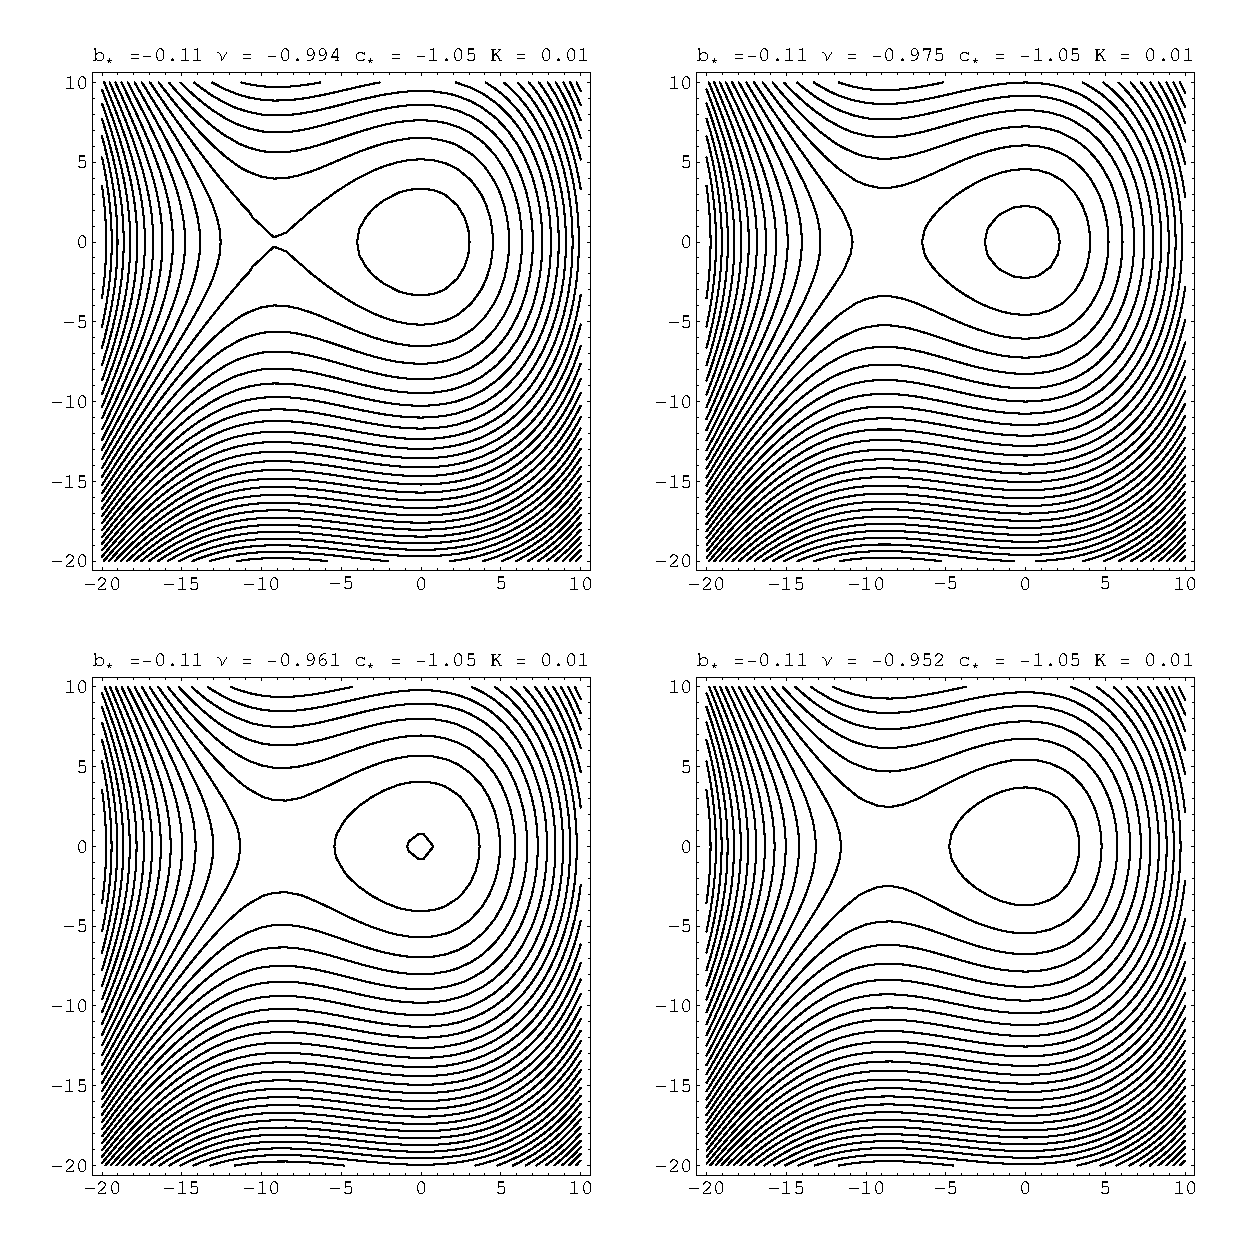
\includegraphics[width=1.0\textwidth]{figures/figure2-1c}
\label{fig:homoclinic2} \caption{Level curves of \eqref{eq:H} corresponding to
various values of H.} \end{center} \end{figure}
